% Created 2025-04-08 Tue 23:06
% Intended LaTeX compiler: pdflatex
\documentclass[11pt]{article}
\usepackage[utf8]{inputenc}
\usepackage[T1]{fontenc}
\usepackage{graphicx}
\usepackage{longtable}
\usepackage{wrapfig}
\usepackage{rotating}
\usepackage[normalem]{ulem}
\usepackage{amsmath}
\usepackage{amssymb}
\usepackage{capt-of}
\usepackage{hyperref}
\usepackage[, slovene]{babel}
\usepackage{float}
\author{Nikola Brković}
\date{\today}
\title{XMPP}
\hypersetup{
 pdfauthor={Nikola Brković},
 pdftitle={XMPP},
 pdfkeywords={},
 pdfsubject={},
 pdfcreator={Emacs 29.4 (Org mode 9.6.15)}, 
 pdflang={Slovene}}
\begin{document}

\maketitle

\section{Namen protokola}
\label{sec:org39d9d94}

XMPP je protokol, namenjen izmenjavi strukturiranih podatkov v
približno realnem času med dvemi ali več entitetami
(Peter Saint-Andre, 2011). Kratica XMPP pomeni \emph{Extensible Messaging and Presence
Protocol}, oziroma v slovenščini - razširljiv protokol sporočil in
prisotnosti.

Čeprav je v teoriji XMPP splošno-namenski protokol za izmenjevanje
sporočil, v praksi se pa največkrat uporablja za hipno sporočanje
(\emph{ang.} \emph{instant messaging} oziroma \emph{IM}) in aplikacije, ki ponujajo
funkcionalnost klepetanja.

\section{Arhitektura protokola}
\label{sec:org61ed453}

Pri arhitekturi protokola so se ustvarjalci protokola XMPP zgledovali
po protokolu SMTP. Udeleženci v protokolu XMPP so povezani v
porazdeljenem omrežju. Vsak udeleženec je bodisi strežnik bodisi
klient. Komunikacija lahko poteka ali med strežniki ali med strežniki
in klienti. En klient je lahko povezan na samo en strežnik in z
drugimi klienti lahko komunicira le posredno prek (enega ali več)
strežnikov.

\section{Scenarij komunikacije}
\label{sec:orge7f4769}

\begin{figure}[H]
\centering
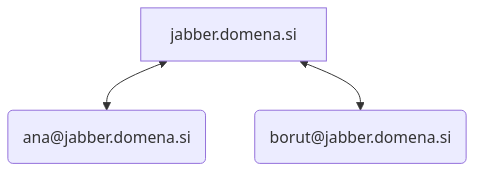
\includegraphics[width=.9\linewidth]{images/local-server.png}
\caption{Komunikacija med uporabniki na istem strežniku}
\end{figure}

\section{Opis specifikacije}
\label{sec:orgc1fc41e}

\section{Format sporočil}
\label{sec:org7fb2390}

\section{Literatura}
\label{sec:org1960d83}

\noindent
Peter Saint-Andre (2011). \emph{{Extensible Messaging and Presence Protocol (XMPP): Core}}, RFC Editor.
\end{document}
